\documentclass{article}

\usepackage[english]{babel}
\usepackage{geometry}
 \geometry{
 a4paper,
 total={170mm,257mm},
 }
\usepackage{graphicx}

\title{Assignment-00 - IsLeapYear function algorithm}
\author{Søren Kastrup}
\date{}

\begin{document}
    \maketitle
    
    \begin{figure}[h]
        \centering
        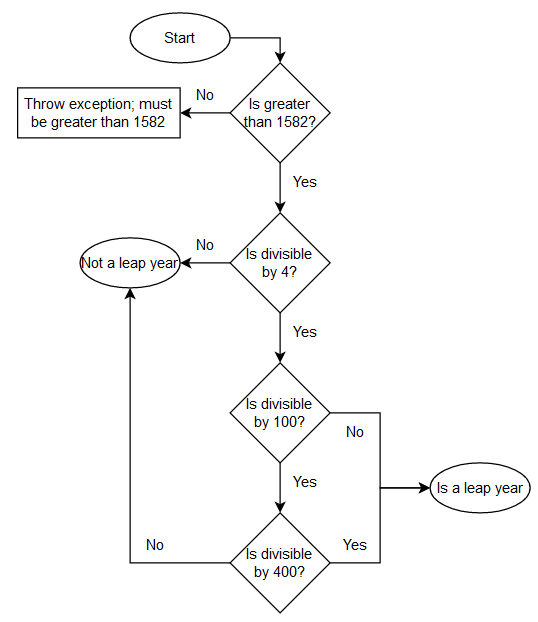
\includegraphics[width=0.6\textwidth]{algorithm_diagram.png}
        \caption{\label{fig:isleapyearalgorithm} A simple UML-diagram displaying the algorithm for the IsLeapYear function.}
    \end{figure}
    
    In the image above the algorithm for the IsLeapYear function is shown by using a UML activity diagram, which describes its workflow in a graphical way. The oval figures represent the start and end, diamonds represent decisions, and rectangles represent exceptions in this case. When the user enters a year into the terminal, by starting in the oval labeled \"start"\ and following the lines in the direction of the arrows depending on the year chosen, it should become clear if it is a leap year or not.

\end{document}